\documentclass[]{article}

%funny text
\usepackage[utf8]{inputenc} % set input encoding (not needed with XeLaTeX)
\usepackage[T1]{fontenc}
\DeclareUnicodeCharacter{00A0}{ }

%packages
\usepackage[english]{babel}
\usepackage[nottoc,notlof,notlot]{tocbibind} % Put the bibliography in the ToC
\usepackage{hyperref} % use hyperlinked ToC
\usepackage{parskip}
\usepackage{booktabs} % for much better looking tables
\usepackage{array} % for better arrays (eg matrices) in maths
\usepackage{paralist} % very flexible & customisable lists (eg. enumerate/itemize, etc.)
\usepackage{verbatim} % adds environment for commenting out blocks of text & for better verbatim
\usepackage{subfig} % make it possible to include more than one captioned figure/table in a single float
\usepackage{listings} %for code listings
\usepackage{color} %for colored syntax highligting
\usepackage{rotating}
\usepackage{pdflscape}
\usepackage[]{algorithm2e}
\usepackage{multirow}
\usepackage{float}
\usepackage{mathtools}
\usepackage{amssymb}
\usepackage{geometry} % to change the page dimensions
\usepackage{indentfirst}
\usepackage[printonlyused]{acronym}
\usepackage[backend=bibtex, bibencoding=utf8]{biblatex}

\graphicspath{ {assets/} }

\bibliography{biblib} 

%%% Page geometry
\geometry{a4paper} % or letterpaper (US) or a5paper or....
\geometry{margin=2.7cm}

%%% Paragraphs and text 
\setlength{\parindent}{4em}
\setlength{\parskip}{1em} 
\renewcommand{\baselinestretch}{1.3}
\setlength{\parskip}{10pt plus 1pt minus 1pt}

%%% Code listing
\definecolor{mygreen}{rgb}{0,0.6,0}
\definecolor{mygray}{rgb}{0.5,0.5,0.5}
\definecolor{mymauve}{rgb}{0.58,0,0.82}
\lstset{
basicstyle=\footnotesize\ttfamily,
commentstyle=\color{mygreen},
keywordstyle=\color{blue},
numberstyle=\tiny\color{mygray},
numbers=left,
tabsize=2,
frame=tb,
aboveskip=3mm,
belowskip=3mm,
breaklines=true,
breakatwhitespace=true,
showstringspaces=false,
columns=flexible
}
% to include a file as a listing: \lstinputlisting{intio.c}
% inline listing: \begin{lstlisting}[frame=single]

\hypersetup{colorlinks=true, linkcolor=black, citecolor=black, filecolor=black, urlcolor=black}

%%%%%%%%%%%%%%%%%%%%%%%%%%%%%%%%%%%%%%%%%%%%%%%%%
%%%%%%%%%%%%%%%%%%%%%%%%%%%%%%%%%%%%%%%%%%%%%%%%%

\title{A Wireless  Low Energy Ambulatory Electroencephalogram}
\author{Thomas Alexander Morrison (tm1810)}
\begin{document}



\begin{titlepage}
% \newgeometry{top=25mm,bottom=25mm,left=38mm,right=32mm}
\setlength{\parindent}{0pt}
\setlength{\parskip}{0pt}
% \fontfamily{phv}\selectfont

{
\Large
\raggedright
Imperial College London\\[17pt]
Department of Electrical and Electronic Engineering\\[17pt]
Final Year Project Report 2014\\[17pt]

}
\rule{\columnwidth}{3pt}

\vfill

\centering
% \includegraphics[width=0.7\columnwidth,height=60mm,keepaspectratio]{imgs/MyRobot.jpg}

\vfill

\setlength{\tabcolsep}{0pt}
\begin{tabular}{p{40mm}p{\dimexpr\columnwidth-40mm}}
Project Title: & \textbf{A Wireless  Low Energy Ambulatory Electroencephalogram} \\[12pt]
Student: & \textbf{Thomas Alexander Morrison} \\[12pt]
CID: & \textbf{00642176} \\[12pt]
Course: & \textbf{ISE4} \\[12pt]
Project Supervisor: & \textbf{James Mardell} \\[12pt]
Second Marker: & \textbf{Dr. Pants Georgiou} \\
\end{tabular}
\end{titlepage}

\clearpage





\clearpage

\section*{Abstract}
Certain neurological medical disorders require continuous monitoring to fully understand and diagnose. Examples of medical interest include epilepsy, syncope, multiple sclerosis, migraines, strokes, Parkinson’s and Alzheimer’s disease. \ac{EEG} is the recording of electrical activity along the scale, resulting from ionic current flows within the neurons of the brain and is useful for both diagnostic and monitoring such aforementioned conditions. Monitoring brain activity can help physicians understand certain characteristics, triggers, and the severity of the disorder. It may be possible to gauge the regions of the brain where the condition is originating and if the patient is a suitable candidate for treatment. 

However, symptoms from neurological disorders often appear sporadically and with little to no warning. Seizures vary from minutes to years apart, and sometimes are not realised or detected without proper equipment. Hospitalising patients for long periods of time is a costly option, and in such circumstances the patient could remain in hospital indefinitely.  Such circumstances lend themselves to an ambulatory system, where an outpatient can be monitored continuously without discomfort or hospitalisation, improving quality of life while decreasing costs. 

With the emergence of low power wireless technologies coupled with portable devices such as tablets and phones, it is a natural technological step to bring care and monitoring out of the hospital and into the home. Through leveraging low energy radio capable platforms, i.e. smartphones and tablets, in the context of an ambulatory EEG, it is possible to empower the patient to inexpensively take health care into their own home and out of the hospital. This project looks at maximising transmission of \ac{EEG} signals over the emerging wireless technology, \ac{BLE}. Further, while this project is targeted at EEG signals, there is no reason why this research and technology cannot be applied to other signals and systems, examples including glucose monitoring, electrocardiography and spirometers.

\cite{Blanco95}
\clearpage
\tableofcontents
\clearpage

%Don't be gay
\section{Acknowledgements}
The opporunity is taken here to express gratitude to all those who have directly contributed towards the project. 

Firstly, the project surperivsors, James Mardell, Chen Guangwei and Esther Rodriguez-Villegas for their. 

Cambridge Silicon Radio providing hardware and technical support. Employees particurarly are Adam Hill, Martin Spikings, Mark Wade, Neil Stewart and Simon. The recently launched uEnergy forum is an excellent source of . CSR also await a report on the speed of 

Guan from NYC

Dr. Nissim Zur, CEO of Vitelix Limited is an expert in low power wireless technologies, and has conversed over many aspects of the final chip used. Further, has also taken an interest in this project's work in regards to maximising the speed, and has requested the results be shared with him.

Finally, and arguarbly most importantly Mike Harbour and Victor Boddy for their efforts in printed circuit board manufacture and assembly. Countless hours were spent in the lab pushing the department's PCB fabrication facilities outside their specifiction and to their limit. 

\clearpage

\section{Introduction}
Patients, however, are unlikely to suffer from neurological disorder while at the clinic as they often appear sporadically during day to day life and with little to no warning. In such circumstances the patient could remain in hospital indefinitely, however seizures can be minutes to years apart, and sometimes are not realised or detected without proper equipment. Such circumstances lend themselves to an ambulatory system, where the patient can be monitored continuously without discomfort or hospitalisation, thus improving quality of life. 



\subsection{Problem Landscape and Motivation}
Neurological disorders and their sequelae are currently estimated to affect upto one seventh of the world's population, a figure which currently stands at 1 billion. With the ever increasing life expectency and decreasing (relative) fertility rates, the population age demographic has shifted towards an ageing population. In tandem, the rates for neurological disorders has increased and is expected to increase further. Diagnosing, monitoring and treating many of these diseases is currently a costly procedure simply due to the time. 

Unfortunately many neurlogical disorder symptons occur sporadically with little to no inidication of an event, such as in the cause of a seizure for epilepsy.



The vast majority of modern smart phones are now being equiped with \ac{BLE} or "Bluetooth Smart" technology. This is a relatively new technology design branded off the popular Bluetooth technology which gained popularity in the early part of last decade. While the two technologies share the same name, their design and operation is very much different. Although origianl Bluetooth's and \ac{BLE}'s use cases may overlap in some scenarios, they were designed to perform well under different circumstances.  

By coupling cheap low power sensors and radios, with powerful ubiquitous consumer technology, it is possible not only to cheaply and efficiently monitor patients, improve the quality of life for patients but also help physicians further their understanding of neurological disorders.

%Smart phone considered high power device anyway. Only hard requirement is that smart phone can support BLE
Currently \ac{BLE} is the only radio technology that is currently being built into all smart phones and tablet devices while offering power consumption low enough to enable a long lifetimes from a lightweight power source. In comparison classic Bluetooth’s power consumption is typically 1 to 2 orders of magnitude higher than BLE. Through leveraging widely popular and familiar smart phone devices with this new technology, in the context of an ambulatory EEG, it is possible to empower the patient to inexpensively take health care into their own home and out of the hospital.


\subsection{Existing Technologies and Products}


With the plethora of emerging low power wireless technologies coupled with portable devices such as tablets and phones, it is a natural technological step to bring care and monitoring out of the hospital and into the home. The consumer fitness sector is being targeted quite strongly, and many devices already exist that utilise lower power technologies to act as gateways for real-time data logging. For example, there already exists a competitive market between heartbeat monitors, cadence monitors and pedometers. These ‘activity trackers’ use low power electronics and radios to log user’s activities and update the user in real time with activity information through the user’s phone or smart watch. Popular products on the market at the time of writing include the Fitbit, Fuelband and Jawbone, which all use the \ac{BLE} technology to connect to smartphones.

\subsection{Project End Goals}
Originally the project was introduced as "Maximising Bluetooth Low Energy throughput of \ac{EEG} signals", however 

Currently, the Imperial College Circuit and System's group has a wired \ac{EEG} measurement device. The wired connection between the EEG sensors and a computer cause patients to remain fairly immobile and hence are impracticable for long periods of use. This project will explore using \ac{BLE} technology for electrocengraphy, and build a prototype system capabale of interfacing with an analouge front to transmit \ac{EEG} data to a portable device such as a tablet or smart phone.  The project will explore the maximum throughput of such a device along with its power consumption.

 At the time of writing, the circuits and systems group at Imperial College have recently taped out a full custom silicon analouge front-end design for manufacture, however these chips will not be available for use before the project deadline. 


Hard requirements of the project include 
\begin{itemize}
	\item Running time of atleast 12 hours
	\item Channel resolution of 8 bits (albeit number of channels undefined)
	\item A weight of less than 10 grams
	\item 10 meter range
	\item BLE wireless technology
	\item Ability to communicate with a smart phone or tablet
\end{itemize}

\subsection {Structure}

\clearpage
\section{Theory and Technology}
\subsection{Bluetooth Low Energy}
The original Bluetooth, hereforth refered to a \ac{BTC}, was intially concieved as the solution to wired communication over short distances (typically less than 100m). The original specification had an air over-the-air rate of 1MBps, though this has increased to around 3 MBps in the latest version of \ac{BTC}. Similarly, BLE has an over-the-air rate of 1MBps. Despite the odd realisation that \ac{BLE}, a much newer technology, has the same over the air rate of last the first incarnation of \ac{BTC}, the maximum theoretical throughput of \ac{BTC} is 700kBps, compared to less than 250kBps for \ac{BLE} - roughly one third of the maximum throughput \ac{BTC} was capable of (the latest version of \ac{BTC} brings the disparity to one ninth). While intuatively it may seem that \ac{BLE} is a less efficient technology, \ac{BLE} can be orders of magnitudes more efficient than \ac{BTC} in particular use cases.

Applications where \ac{BLE} excels in are ones where communication between two devices is only required intermitently, and the volume of information sent is small. An example would be a thermometer in a greenhouse connected by radio to a visual display unit inside the home. Temperature changes at a rate slow enough that it is only necessary to check the temperature every 10 minutes. Once every 10 minutes the radio thermometer device can wake up take a measurement, send a notification of a measurement then return to a deep sleep. \ac{BLE} does this much better than \ac{BTC}, taking only a few milliseconds to connect. \ac{BTC} takes between a few hundred milliseconds to several seconds to reconnect. While both millisecond orders of magnitude and second orders of magnitude are small when compared to an order of magnitude of minutes, over time it adds up to a significant amount, and \ac{BLE} devices can last many years of a small, single coin cell. \ac{BLE} is excellent for applications which involve small episodic transmission of data. In the scenario described a \ac{BTC} system would have a lifetime of approximately 100 days from a typical 3v lithium cell. Off the same cell, a \ac{BLE} system would have a lifetime of many years. In fact, in this scenario the \ac{BLE} system lifetime can be extended further as \ac{BLE} can support connectionless communication, whereby it simply wakes up and transmits the thermometer state to any device that's listening without the need for acknowledgement.

The reason the reconnection times are much faster for \ac{BLE} is as far as the communication devices are concerned, they never disconnected. Rather in the \ac{BLE} protocol, the devices agree to meet a specified periods known as \ac{CI}. The devices are free to perform any operations in the mean time, though typically enter a state of hibernation. In many scenarios between two radios, one device will be much more power conscious. In the example above, the battery powered device in the greenhouse would typically be the power conscious device while the visual disuplay unit inside the home will likely be powered from the grid, and have no concern as to its power consupmption. In these situations, we define the power conscious device to be the slave and the remaining device to be the master. 

The slave device also has the ability to skip connection intervals. That is, the slave to skip a upto a predetermined number of connection intervals, known as the slave latency. While the master must always check back to see if the slave has sent anything, the slave, if it has nothing to send, doesn't need to wake up. For example, if the slave latency is 120, and the connection interval is 1000ms, then the slave is not obliged to communicate with the master for upto 2 minutes, despite the master having to check every 1000ms. If the slave is not able to make contact with the master after 2 minutes, then the master will begin counting the number of times the slave has missed the obliged connection period (that is the \ac{CI} multiplied by the time slave latency). If this value reaches above a certain threshold (a typically recommened value of 6), the master will consider the slave disconnected, and be required to go through a connection process again[UNLESS USING BROADCASTING TO SEND DATA]. Continuing with the scenario, the slave will be considered disconnected if it hasn't made contact with the master after 12 minutes.

Another contribution to reduced power over \ac{BTC} is the reduction in the number of channels used in communicaton. \ac{BTC}, \ac{BLE} along with other wireless technologies that operate in the 2.4GHz ISM band such as a WiFi and ZigBee all make use of spread spectrum techniques to achieve a sufficient level of noise immunity. That is, the available bandwidth is split (spread) into smaller channels and radios communicate between one another using a pre-dertmined channel hop sequence. As the number of channels decreases, the channel band size grows requiring less accurate and complex modulation hardware, hence decreasing power consumption. \ac{BTC} originally used 79 channels, and \ac{BLE} reduces this to 39.

\begin{figure}[htb]
	\begin{center}
		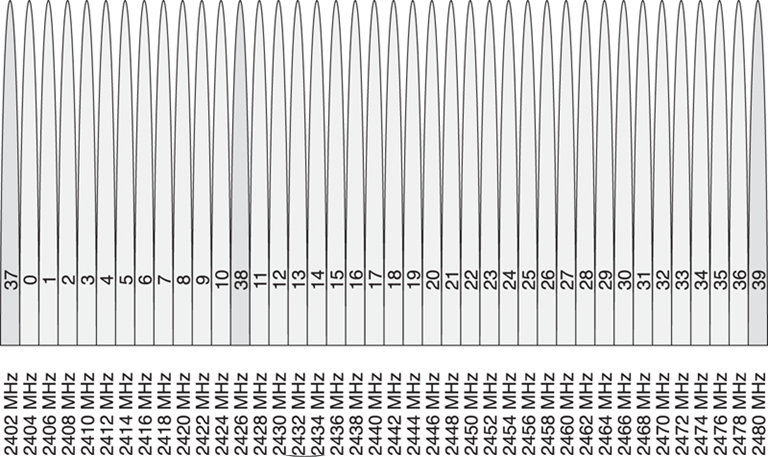
\includegraphics[width = 0.7\textwidth]{blechannels}
	\end{center}
	\caption{\ac{BLE} channels (advertisement channels render darker)}
	\label{fig:blechannels}
\end{figure}

\begin{figure}[htb]
	\begin{center}
		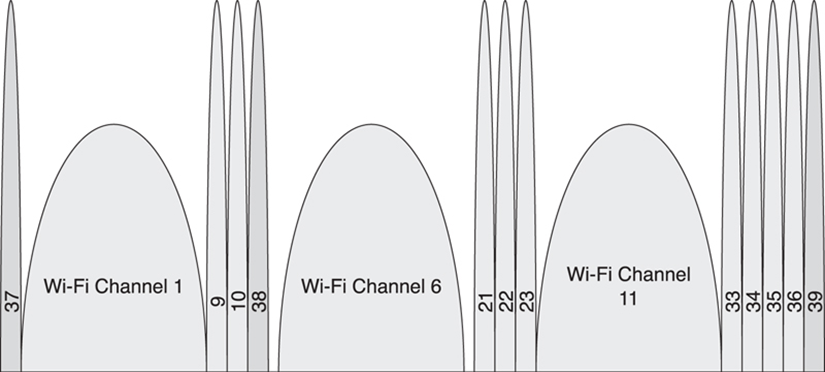
\includegraphics[width = 0.7\textwidth]{blechannelswifi}
	\end{center}
	\caption{\ac{BLE} channels with WiFi channels overlaid}
	\label{fig:blechannelswifi}
\end{figure}


The number of channels dedicated to advertising has also decreased, meaing less time is spent searching for discoverable devices. The advertisement channels have been specifically chosen not to interfere with the common WiFi channels. Finally, the radio characteristics are very dependent on temperature. Complex mechanisms are used to compensate and recalibrate on-the-fly radio parameters. Due to the episodic nature of \ac{BLE} the radio does not come under such thermal extremes. All these design changes have positive hardware ramifications. The reduced compelxity of \ac{BLE} means reduced hardware requirements (notably memory), in turn reducing the leakage current. 

\ac{BTC} was designed with the idea that it would be used to do many common jobs, and hence particular configurations were built into it. In \ac{BTC}, these configurations are known as profiles. Example profiles include the audio distribution profile (A2DP), which is used in by many Bluetooth product manufacturers to allow a device, such as a phone to interact with an audio system, such as in a car. Another example would be the serial port profile (SPP), meant to emulate the highly popular and robust RS-232 serial standard for data transfer (recall that \ac{BTC} was concieved as a solution to wires). This is all built into what is known as the Bluetooth stack – a software framework that interacts between the physical layer and the application layer\footnote{Depending on what level of the stack one is working, master can take the names central or client, while slave can take peripheral or server.}.  

\ac{BLE} also makes use of this paradigm but is often superficially depicted as \ac{BTC} operating at lower speeds and power consumption. It is not currently compatible with \ac{BTC} and there are no plans for it to be. Like \ac{BTC}, the \ac{BLE} architecture has 3 over-arching parts: Application, Host and Controller. The controller, simply put, is the radio and related hardware controllers and the application the use case, which could be a cadence monitor, thermometer or even an electroencephalogram. It is the host controller interface (HCI), commonly known as the “stack” that provides the necessary software to enable the application layer to communicate with the radio (see Figure~\ref{fig:ble_arch}).

\begin{figure}[htb]
	\begin{center}
		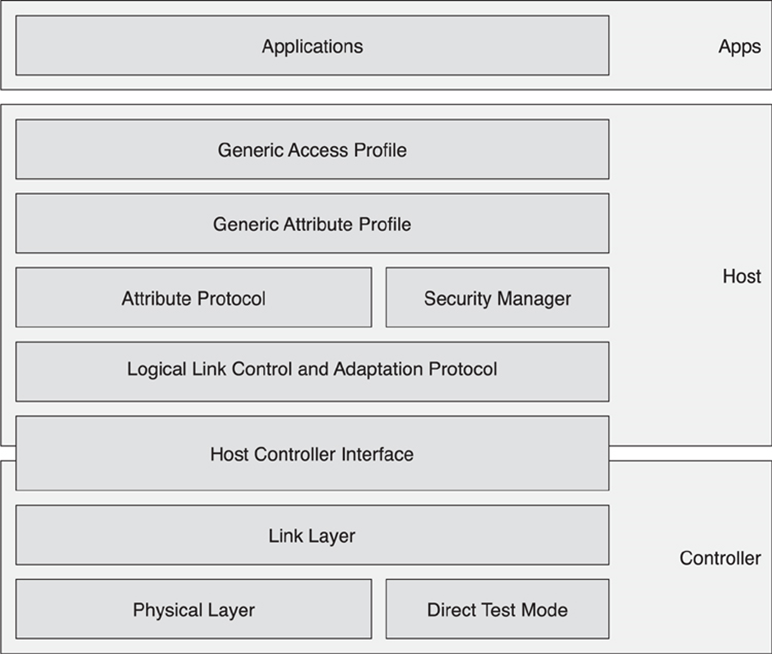
\includegraphics[width = 0.7\textwidth]{ble_arch}
	\end{center}
	\caption{\ac{BLE} Architecture}
	\label{fig:ble_arch}
\end{figure}

In an attempt to be economical with time and space components of the stack deemed irrelevant will not be discussed further here. For example a description of the security manager is not relevant as this project is not concerned with sending data over encrypted links. Similarly, the Logical Link Control and Adaption Protocol, while used extenivesly in all radio communication will not be discussed in detail as it doesn't provide any insight into maximising throughput or minimising power.

In \ac{BTC} profiles were diverse and large enough to warrant chip designers releasing tailored chips to perform well for a specific profile, i.e. a chip supporting A2DP may contain \ac{CODEC} hardware for real time audio streaming. In \ac{BLE} the profile framework is far lighter. \ac{BLE}'s profiles are all built ontop of  the \ac{GATT}, which in turn is built upon the \ac{ATT}, a protocol optimised to run on BLE devices. Attributes are an umbrella term, being the atomic unit of data communicated between BLE devices. Profiles are hierarchical constructions of attributes, in the top down order of profile, service, characteristic and descriptors, as shown in Figure~\ref{fig:exampleprofile}. A BLE device implements atleast one profile, \ac{GAP} along one more which is typically the purpose of the device. \ac{GAP} contains important information such the the device name and prefered connection properties.  This second profile can be one of the standard profiles as defined by the SIG group or a bespoke profile for the application, such as the case for a \ac{EEG}. Popular, SIG defined examples of \ac{BLE} profiles include the heart rate profile (HRP), health thermometer profile (HTP) and even a glucose profile (GLP) with room for many more to be incorporated into the core \ac{BLE} \ac{SIG} defined \ac{GATT} specifications.  

\begin{figure}[htb]
	\begin{center}
		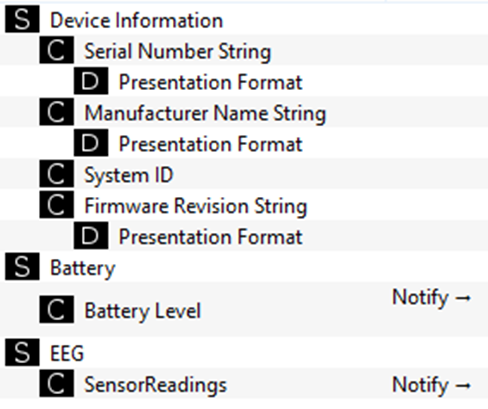
\includegraphics[width = 0.5\textwidth]{exampleprofile}
	\end{center}
	\caption{Example GATT profile consisting of 12 attribute - 3 services, 6 characteristics and 3 descriptors. }
	\label{fig:exampleprofile}
\end{figure}

 Attributes represent information about state. In the case of the greenhouse, the state would include the measured temperature. A suitable profile name which encapsulates the state is ''thermometer'', which contains the services ''device information'', ''battery service'', and ''thermometer''. As in figure~\ref{fig:exampleprofile}, the greenhouse thermometer service may contain the same device information and battery services, but replace the ''EEG'' service with the thermometer service, and the ''SensorReadings'' service with temperature. The other profile, \ac{GAP}, will contain the attributes which define how \ac{BLE} unit discover and establish connection to one another.  This includes the device name, perhaps ''greenhouse thermometer'', along with the preferred slave connection properties, e.g. a connection interval of 4 seconds, with a slave latency of 150 (10 minute window). All this information is contained within the GATT database, and shared as needed to other \ac{BLE} units. 

When communicating attributes, there are four data operations available. Read and write typically require one device to access the others characteristic. In the case of the greenhouse, the house device would request to read the thermometer. Notification and indications differ to read and write, in that the device(s) after information subscribes to the changes of state of the characteristics. For example, when greenhouse slave device wakes up, if the thermometer measurement changed, it will send a notification or indication alert the master device inside the house. The former methods can be thought of as synchronous means of communication while the latter asynchronous. Notifications differ from indications in that indications require a application level acknowledgment. That is, the indication is bubbled up to the user code, which then either accepts or rejects the indications. Notifications are acknowledge near the bottom of the \ac{BLE} stack, verifying correct receipt and message integrity. Therefore notifications are suitable for higher throughput applications. As shown in figure~\ref{fig:exampleprofile} shows notifications are operation configured for battery and EEG sensor readings. In this example, whenever the battery level changes, any devices subscribed to the characteristic battery level will receive a notification.

In \ac{BTC} the network topology used pico-nets, whereby one device has one master, but could be a master of another device. \ac{BLE} operates a simpler network topology, star, whereby a device can either be a master or slave, but not both. The master has the responsibility of organising itself between the slaves. If one slave requires large amounts of bandwidth, it my impact the quality of service encountered by the other devices. 

\begin{figure}[htb]
	\begin{center}
		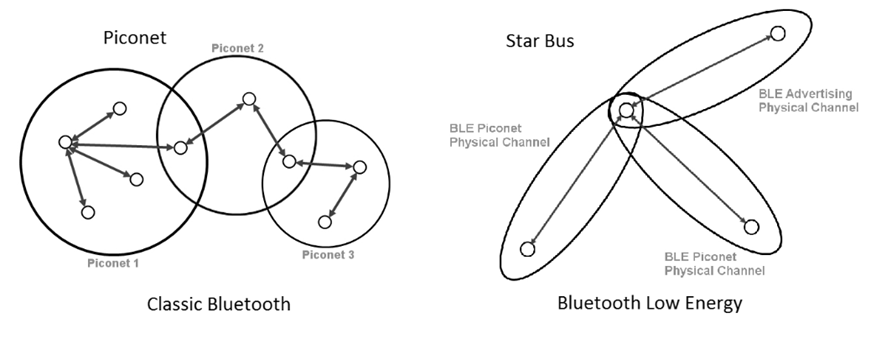
\includegraphics[width = \textwidth]{topology}
	\end{center}
	\caption{Bluetooth Network Topologies }
	\label{fig:topology}
\end{figure}

Both BLE and BTC devices move through generic system states. The same abstract view can be applied to both technologies and is shown in. Note that depending on the role of the device, the state moves right (master) or left (slave) from standby. It may appearing confusing to have another state for scanning which can only move into the standby state, but this is useful for searching and discovering devices with no commitment to connecting. Such a use case might be suitable for devices that intermittently broadcast small amounts of information. Assuming that the master BLE device is in the initiating state, searching for a connectable device, and at the same time the BLE slave is in the advertising stage, periodically broadcasting information using advertisement packets; the two devices will find one another and may initiate a connection request.

\begin{figure}[htb]
	\begin{center}
		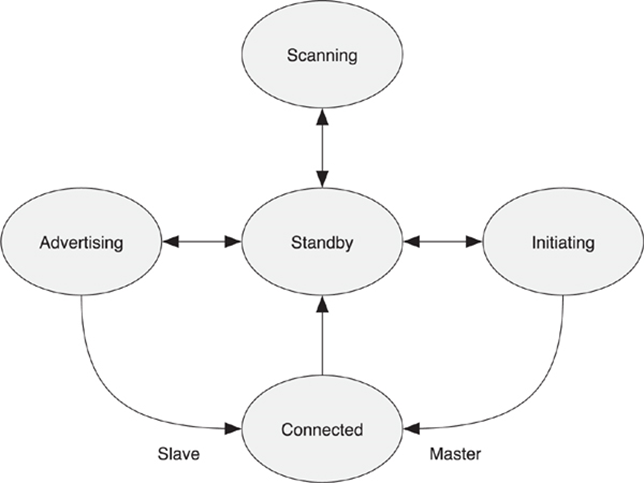
\includegraphics[width = 0.8\textwidth]{systemstate}
	\end{center}
	\caption{Device State Transition Diagram}
	\label{fig:systemstate}
\end{figure}


\clearpage

\section{Preliminary Research}

This section deals with evaluating the technology and radios

\subsection{Radio Evaluation}

There are a number of competing companies int the \ac{BLE} consume space. The most popular chip manufacturers at the time of evaluation are\ac{TI}, \ac{NS} and \ac{CSR}, although  other manufacturers exist, they normally design multi-wireless technology chips, e.g. Broadcomm, which support WiFi, \ac{BTC} and \ac{BLE}. These chips are not suitable for this project due to their complexity, intend application (. The typical use case of such combo-chips are in tablets, smartphones and notebooks. There

After sourcing
\subsubsection{nRF8001}
The first radio tested was \ac{NS}'s nRF8001, selected due to the data sheet claiming it was the lowest power consuming device. The reason for this was because the chip only contained a controller and host layer. The application layer must be provided by an external micro controller, which is a large amount of effort to write. Fortunately a hobbyist open source project\cite{Guan2013} was available that provided the necessary code to get limited connectivity up and running.

Using a shunt resistor, the measured peak current was approximately 14.5mA, which correlates well with the data sheet specification of 14.6mA. This was at a 

The ATMega328 consumes approximately XmA, however for the remainder. As the device was hardware limited to only 1 packet per connection event further development was abandoned


\cite{nrf8001}

\begin{figure}[htb]
	\begin{center}
		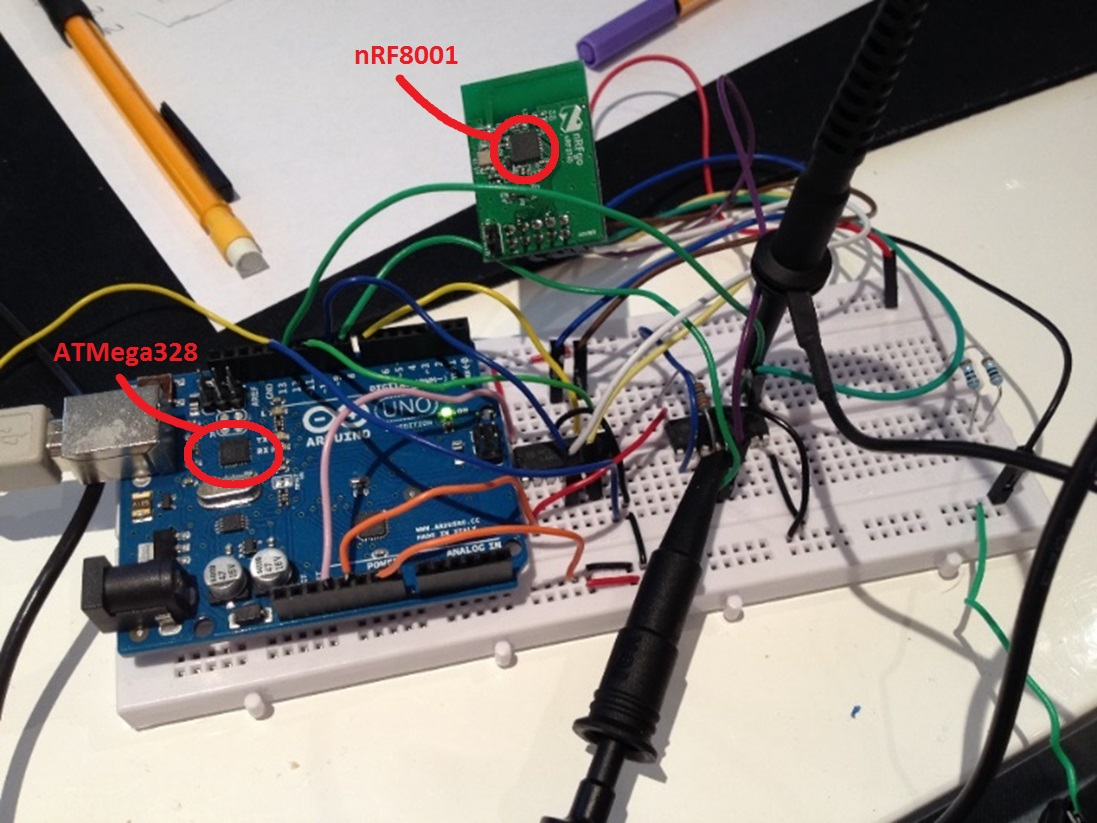
\includegraphics[width = 0.8\textwidth]{nrf8001}
	\end{center}
	\caption{Arduino Uno development board acting hosting the application layer for the nRF8001 radio. Level shifters were required for interfacing with the low-paper chip}
	\label{fig:nrf8001}
\end{figure}

The first radio tested was \ac{TI}'s CC2541 as part of the sensor tag package 
\subsection{Component Selection}

\section{Specification}

\section{Prototype Design}

\section{Results}

\section{Evaluation}

\subsection{Power Analysis}

\subsection{Bill of materials}

\section{Conclusions and Future Work}
On the whole, the project has 

Not all tablets will be able to run at full speed

Ideally, it is desirable to write a conference style paper. 

Useful for CSR
\section{Final Remarks}
A vast array of technologies and tools were used throughout this project. Below highlights those that are non-trivial and were of significant importance

\begin{itemize}
	\item Git verisioning control - For versioning and segmenting the workflow
	\item xIDE - CSRs integrated development suite for compiling and debugging CSR-stack based chips. This is where the firmware for the CSR1010 MCU was written
	\item Wireshark - Invaluable in analysing the packets and control flow between BLE radios, unfortunately must be used offline
	\item SmartRF online packet sniffer - Useful as a low-speed packet sniffer. Extremely useful in the early days of the project, however the throughputs eventually obtained rendered the tool and hardware redundant as it was not capable of such speeds
	\item Visual Studio 2013 - Primairly used for developing the tablet application. Highly useful for "knocking up" quick throughput expirements 
\end{itemize}

The large amount of both written and generated code is to vast to warrant being included in this report. Therefore is has been decided to make it publically available online at the git repositry address 
\url{https://github.com/proftom/AmbulatoryEEG}.

\section{Bibliography}
\clearpage

\nocite{*}

\printbibliography


\section{Appendix}
\subsection{Acronyms}
\begin{acronym}
	\acro{EEG}{Electroencephalography}
	\acro{BLE}{Bluetooth Low Energy}
	\acro{BTC}{Bluetooth Classic}
	\acro{CSR}{Cambridge Silicon Radio}
	\acro{TI}{Texas Instruments}
	\acro{NS}{Nordic Semiconductor}
	\acro{GATT}{Generic Attribute Profile}
	\acro{GAP}{Generic Access Profile}
	\acro{ATT}{Attribute Protocol}
	\acro{CI}{connection interval}
	\acro{SIG}{Special Interests Group}
	\acro{CODEC}{coder/decoder}
\end{acronym}

\section{User Guide}
\end{document}